%% LaTeX2e class for student theses
%% sections/apendix.tex
%% 
%% Karlsruhe Institute of Technology
%% Institute of Information Security and Dependability
%% Software Design and Quality (SDQ)
%%
%% Dr.-Ing. Erik Burger
%% burger@kit.edu
%%
%% Version 1.5, 2024-02-12

\iflanguage{english}
{\chapter{Appendix}}    % english style
{\chapter{Anhang}}      % german style
		
\setcounter{figure}{0}
		
\begin{figure}[ht]
  \centering
  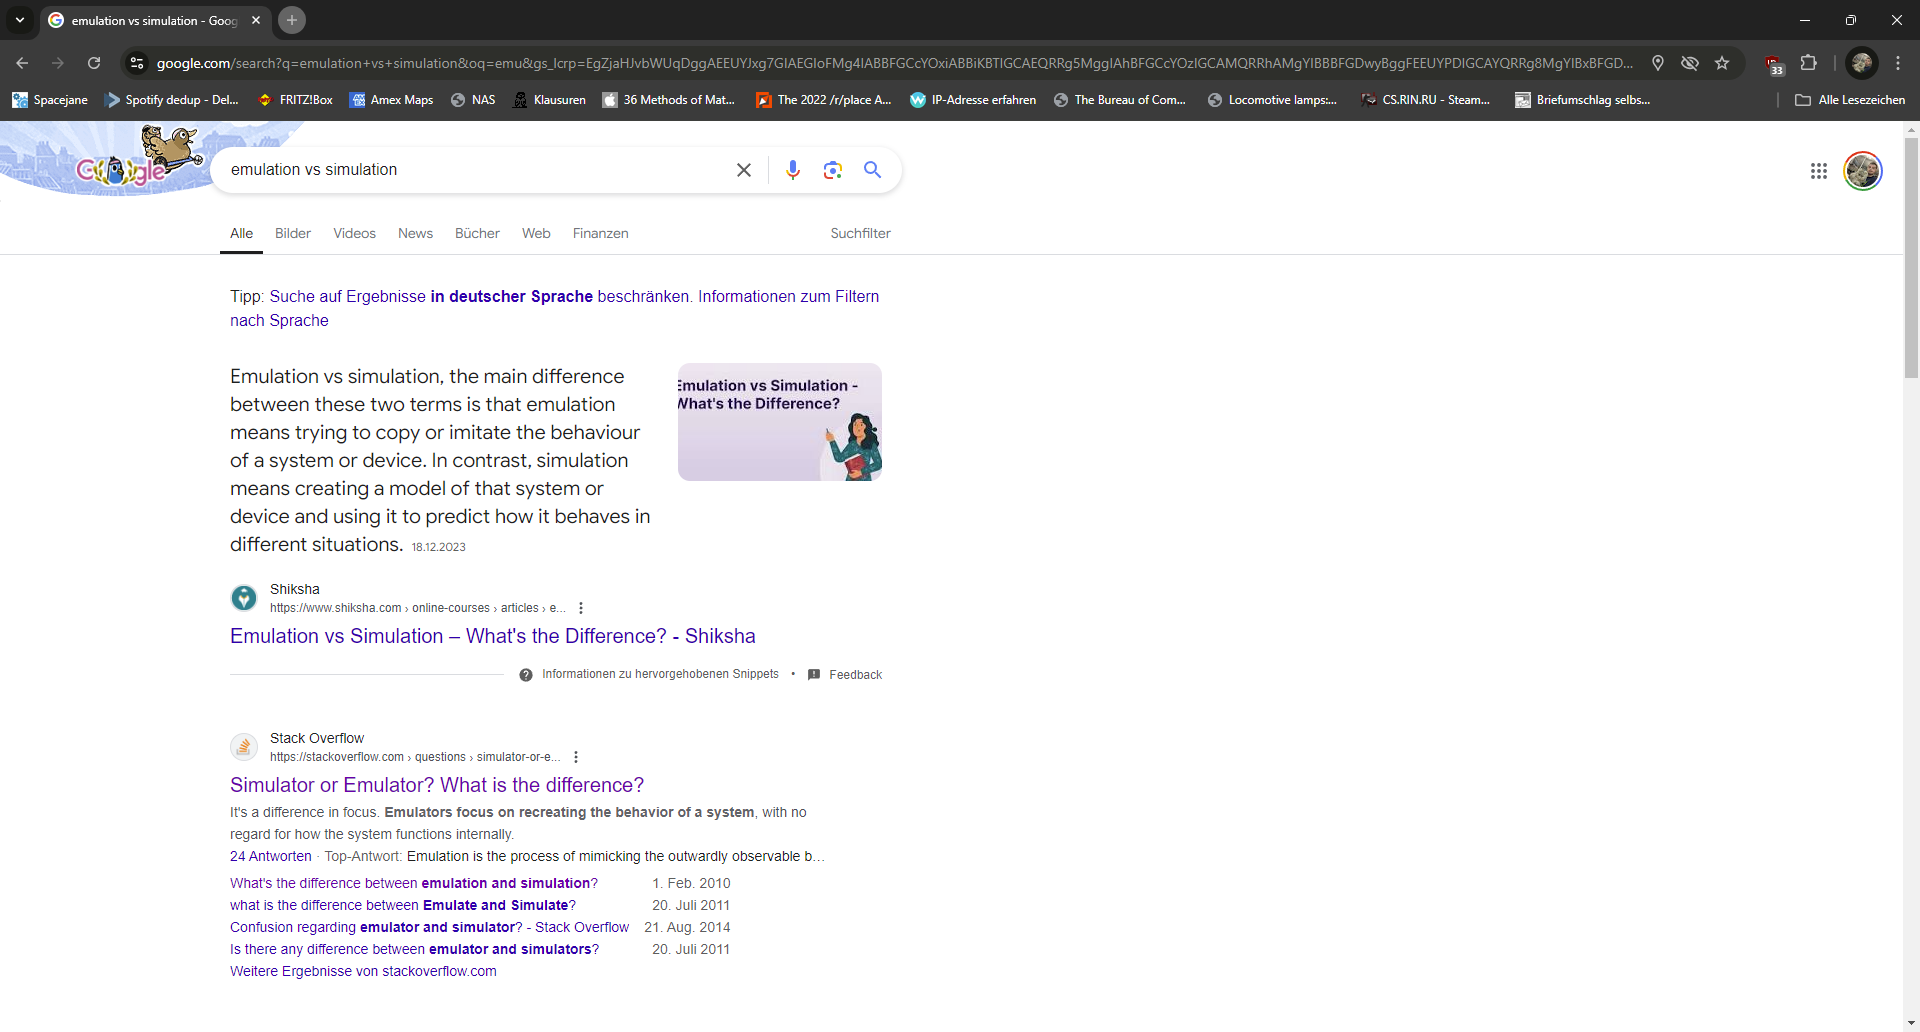
\includegraphics[width=\textwidth]{images/StackOverflow}
  \caption{Results when searching the difference between Simulation and Emulation.}
  \label{fig:Google_SO}
\end{figure}

\newgeometry{left=1cm,right=1cm}

\begin{figure}[ht]
  \tiny
  \centering
  \begin{minipage}{0.48\linewidth}
  \begin{ffcode}
    address-space: I/O
      0000000000000000-000000000000ffff (prio 0, i/o): io

    address-space: gpex-root
      0000000000000000-ffffffffffffffff (prio 0, i/o): bus master container

    address-space: virtio-gpu-pci
      0000000000000000-ffffffffffffffff (prio 0, i/o): bus master container

    address-space: cpu-memory-0
    address-space: memory
      0000000000000000-ffffffffffffffff (prio 0, i/o): system
        0000000000000000-0000000003ffffff (prio 0, romd): virt.flash0
        0000000004000000-0000000007ffffff (prio 0, romd): virt.flash1
        0000000008000000-0000000008000fff (prio 0, i/o): gic_dist
        0000000008010000-0000000008011fff (prio 0, i/o): gic_cpu
        0000000008020000-0000000008020fff (prio 0, i/o): gicv2m
        0000000009000000-0000000009000fff (prio 0, i/o): pl011
        0000000009010000-0000000009010fff (prio 0, i/o): pl031
        0000000009020000-0000000009020007 (prio 0, i/o): fwcfg.data
        0000000009020008-0000000009020009 (prio 0, i/o): fwcfg.ctl
        0000000009020010-0000000009020017 (prio 0, i/o): fwcfg.dma
        0000000009070000-0000000009070017 (prio 0, i/o): memhp container
        0000000009080000-0000000009080003 (prio 0, i/o): acpi-ged
        000000000a000000-000000000a0001ff (prio 0, i/o): virtio-mmio
        000000000a000200-000000000a0003ff (prio 0, i/o): virtio-mmio
        000000000a000400-000000000a0005ff (prio 0, i/o): virtio-mmio
        000000000a000600-000000000a0007ff (prio 0, i/o): virtio-mmio
        000000000a000800-000000000a0009ff (prio 0, i/o): virtio-mmio
        000000000a000a00-000000000a000bff (prio 0, i/o): virtio-mmio
        000000000a000c00-000000000a000dff (prio 0, i/o): virtio-mmio
        000000000a000e00-000000000a000fff (prio 0, i/o): virtio-mmio
        000000000a001000-000000000a0011ff (prio 0, i/o): virtio-mmio
        000000000a001200-000000000a0013ff (prio 0, i/o): virtio-mmio
        000000000a001400-000000000a0015ff (prio 0, i/o): virtio-mmio
        000000000a001600-000000000a0017ff (prio 0, i/o): virtio-mmio
        000000000a001800-000000000a0019ff (prio 0, i/o): virtio-mmio
        000000000a001a00-000000000a001bff (prio 0, i/o): virtio-mmio
        000000000a001c00-000000000a001dff (prio 0, i/o): virtio-mmio
        000000000a001e00-000000000a001fff (prio 0, i/o): virtio-mmio
        000000000a002000-000000000a0021ff (prio 0, i/o): virtio-mmio
        000000000a002200-000000000a0023ff (prio 0, i/o): virtio-mmio
        000000000a002400-000000000a0025ff (prio 0, i/o): virtio-mmio
        000000000a002600-000000000a0027ff (prio 0, i/o): virtio-mmio
        000000000a002800-000000000a0029ff (prio 0, i/o): virtio-mmio
        000000000a002a00-000000000a002bff (prio 0, i/o): virtio-mmio
        000000000a002c00-000000000a002dff (prio 0, i/o): virtio-mmio
        000000000a002e00-000000000a002fff (prio 0, i/o): virtio-mmio
        000000000a003000-000000000a0031ff (prio 0, i/o): virtio-mmio
        000000000a003200-000000000a0033ff (prio 0, i/o): virtio-mmio
        000000000a003400-000000000a0035ff (prio 0, i/o): virtio-mmio
        000000000a003600-000000000a0037ff (prio 0, i/o): virtio-mmio
        000000000a003800-000000000a0039ff (prio 0, i/o): virtio-mmio
        000000000a003a00-000000000a003bff (prio 0, i/o): virtio-mmio
        000000000a003c00-000000000a003dff (prio 0, i/o): virtio-mmio
        000000000a003e00-000000000a003fff (prio 0, i/o): virtio-mmio
        000000000c000000-000000000dffffff (prio 0, i/o): platform bus
        0000000010000000-000000003efeffff (prio 0, i/o): alias pcie-mmio @gpex_mmio_window 0000000010000000-000000003efeffff
        000000003eff0000-000000003effffff (prio 0, i/o): gpex_ioport_window
          000000003eff0000-000000003effffff (prio 0, i/o): gpex_ioport
        0000000040000000-00000000bfffffff (prio 0, ram): mach-virt.ram
        0000004010000000-000000401fffffff (prio 0, i/o): alias pcie-ecam @pcie-mmcfg-mmio 0000000000000000-000000000fffffff
        0000008000000000-000000ffffffffff (prio 0, i/o): alias pcie-mmio-high @gpex_mmio_window 0000008000000000-000000ffffffffff
    \end{ffcode}
    \end{minipage}
    \begin{minipage}{0.48\linewidth}
    \begin{ffcode}
    address-space: virtio-net-pci
      0000000000000000-ffffffffffffffff (prio 0, i/o): bus master container

    memory-region: system
      0000000000000000-ffffffffffffffff (prio 0, i/o): system
        0000000000000000-0000000003ffffff (prio 0, romd): virt.flash0
        0000000004000000-0000000007ffffff (prio 0, romd): virt.flash1
        0000000008000000-0000000008000fff (prio 0, i/o): gic_dist
        0000000008010000-0000000008011fff (prio 0, i/o): gic_cpu
        0000000008020000-0000000008020fff (prio 0, i/o): gicv2m
        0000000009000000-0000000009000fff (prio 0, i/o): pl011
        0000000009010000-0000000009010fff (prio 0, i/o): pl031
        0000000009020000-0000000009020007 (prio 0, i/o): fwcfg.data
        0000000009020008-0000000009020009 (prio 0, i/o): fwcfg.ctl
        0000000009020010-0000000009020017 (prio 0, i/o): fwcfg.dma
        0000000009070000-0000000009070017 (prio 0, i/o): memhp container
        0000000009080000-0000000009080003 (prio 0, i/o): acpi-ged
        000000000a000000-000000000a0001ff (prio 0, i/o): virtio-mmio
        000000000a000200-000000000a0003ff (prio 0, i/o): virtio-mmio
        000000000a000400-000000000a0005ff (prio 0, i/o): virtio-mmio
        000000000a000600-000000000a0007ff (prio 0, i/o): virtio-mmio
        000000000a000800-000000000a0009ff (prio 0, i/o): virtio-mmio
        000000000a000a00-000000000a000bff (prio 0, i/o): virtio-mmio
        000000000a000c00-000000000a000dff (prio 0, i/o): virtio-mmio
        000000000a000e00-000000000a000fff (prio 0, i/o): virtio-mmio
        000000000a001000-000000000a0011ff (prio 0, i/o): virtio-mmio
        000000000a001200-000000000a0013ff (prio 0, i/o): virtio-mmio
        000000000a001400-000000000a0015ff (prio 0, i/o): virtio-mmio
        000000000a001600-000000000a0017ff (prio 0, i/o): virtio-mmio
        000000000a001800-000000000a0019ff (prio 0, i/o): virtio-mmio
        000000000a001a00-000000000a001bff (prio 0, i/o): virtio-mmio
        000000000a001c00-000000000a001dff (prio 0, i/o): virtio-mmio
        000000000a001e00-000000000a001fff (prio 0, i/o): virtio-mmio
        000000000a002000-000000000a0021ff (prio 0, i/o): virtio-mmio
        000000000a002200-000000000a0023ff (prio 0, i/o): virtio-mmio
        000000000a002400-000000000a0025ff (prio 0, i/o): virtio-mmio
        000000000a002600-000000000a0027ff (prio 0, i/o): virtio-mmio
        000000000a002800-000000000a0029ff (prio 0, i/o): virtio-mmio
        000000000a002a00-000000000a002bff (prio 0, i/o): virtio-mmio
        000000000a002c00-000000000a002dff (prio 0, i/o): virtio-mmio
        000000000a002e00-000000000a002fff (prio 0, i/o): virtio-mmio
        000000000a003000-000000000a0031ff (prio 0, i/o): virtio-mmio
        000000000a003200-000000000a0033ff (prio 0, i/o): virtio-mmio
        000000000a003400-000000000a0035ff (prio 0, i/o): virtio-mmio
        000000000a003600-000000000a0037ff (prio 0, i/o): virtio-mmio
        000000000a003800-000000000a0039ff (prio 0, i/o): virtio-mmio
        000000000a003a00-000000000a003bff (prio 0, i/o): virtio-mmio
        000000000a003c00-000000000a003dff (prio 0, i/o): virtio-mmio
        000000000a003e00-000000000a003fff (prio 0, i/o): virtio-mmio
        000000000c000000-000000000dffffff (prio 0, i/o): platform bus
        0000000010000000-000000003efeffff (prio 0, i/o): alias pcie-mmio @gpex_mmio_window 0000000010000000-000000003efeffff
        000000003eff0000-000000003effffff (prio 0, i/o): gpex_ioport_window
          000000003eff0000-000000003effffff (prio 0, i/o): gpex_ioport
        0000000040000000-00000000bfffffff (prio 0, ram): mach-virt.ram
        0000004010000000-000000401fffffff (prio 0, i/o): alias pcie-ecam @pcie-mmcfg-mmio 0000000000000000-000000000fffffff
        0000008000000000-000000ffffffffff (prio 0, i/o): alias pcie-mmio-high @gpex_mmio_window 0000008000000000-000000ffffffffff

    memory-region: gpex_mmio_window
      0000000000000000-ffffffffffffffff (prio 0, i/o): gpex_mmio_window
        0000000000000000-ffffffffffffffff (prio 0, i/o): gpex_mmio

    memory-region: pcie-mmcfg-mmio
      0000000000000000-000000000fffffff (prio 0, i/o): pcie-mmcfg-mmio
  \end{ffcode}
  \end{minipage}
  \caption{Full output of \emph{info mtree} on a 2GB ARM64 instance.}
  \label{fig:mem_ARM_full}
\end{figure}

\begin{figure}
  \tiny
  \begin{minipage}{0.48\linewidth}
    \begin{ffcode}
    address-space: piix3-ide
      0000000000000000-ffffffffffffffff (prio 0, i/o): bus master container
        0000000000000000-ffffffffffffffff (prio 0, i/o): alias bus master @system 0000000000000000-ffffffffffffffff

    address-space: pci-ohci
      0000000000000000-ffffffffffffffff (prio 0, i/o): bus master container
        0000000000000000-ffffffffffffffff (prio 0, i/o): alias bus master @system 0000000000000000-ffffffffffffffff

    address-space: xbox-lpc
      0000000000000000-ffffffffffffffff (prio 0, i/o): bus master container

    address-space: pci-testdev
      0000000000000000-ffffffffffffffff (prio 0, i/o): bus master container

    address-space: mcpx-aci
      0000000000000000-ffffffffffffffff (prio 0, i/o): bus master container
        0000000000000000-ffffffffffffffff (prio 0, i/o): alias bus master @system 0000000000000000-ffffffffffffffff

    address-space: I/O
      0000000000000000-000000000000ffff (prio 0, i/o): io
        0000000000000000-0000000000000fff (prio 1, i/o): alias pci_bridge_io @pci_bridge_io 0000000000000000-0000000000000fff
        0000000000000000-0000000000000007 (prio 0, i/o): dma-chan
        0000000000000008-000000000000000f (prio 0, i/o): dma-cont
        0000000000000020-0000000000000021 (prio 0, i/o): pic
        0000000000000040-0000000000000043 (prio 0, i/o): pit
        0000000000000061-0000000000000061 (prio 0, i/o): pcspk
        0000000000000070-0000000000000073 (prio 0, i/o): rtc
          0000000000000070-0000000000000070 (prio 0, i/o): rtc-index
        000000000000007e-000000000000007f (prio 0, i/o): kvmvapic
        0000000000000081-0000000000000083 (prio 0, i/o): dma-page
        0000000000000087-0000000000000087 (prio 0, i/o): dma-page
        0000000000000089-000000000000008b (prio 0, i/o): dma-page
        000000000000008f-000000000000008f (prio 0, i/o): dma-page
        00000000000000a0-00000000000000a1 (prio 0, i/o): pic
        00000000000000c0-00000000000000cf (prio 0, i/o): dma-chan
        00000000000000d0-00000000000000df (prio 0, i/o): dma-cont
        0000000000000170-0000000000000177 (prio 0, i/o): ide
        00000000000001f0-00000000000001f7 (prio 0, i/o): ide
        0000000000000376-0000000000000376 (prio 0, i/o): ide
        00000000000003f6-00000000000003f6 (prio 0, i/o): ide
        00000000000004d0-00000000000004d0 (prio 0, i/o): elcr
        00000000000004d1-00000000000004d1 (prio 0, i/o): elcr
        0000000000000cf8-0000000000000cfb (prio 0, i/o): pci-conf-idx
        0000000000000cfc-0000000000000cff (prio 0, i/o): pci-conf-data
        0000000000008000-00000000000080ff (prio 1, i/o): xbox-pm
          0000000000008000-0000000000008003 (prio 0, i/o): acpi-evt
          0000000000008004-0000000000008005 (prio 0, i/o): acpi-cnt
          0000000000008008-000000000000800b (prio 0, i/o): acpi-tmr
          0000000000008020-0000000000008023 (prio 0, i/o): xbox-pm-gpe0
          00000000000080c0-00000000000080d9 (prio 0, i/o): xbox-pm-gpio
        000000000000c000-000000000000c01f (prio 1, i/o): xbox-smbus-bar
        000000000000e000-000000000000e007 (prio 1, i/o): nvnet-io
        000000000000ff60-000000000000ff6f (prio 1, i/o): piix-bmdma-container
          000000000000ff60-000000000000ff63 (prio 0, i/o): piix-bmdma
          000000000000ff64-000000000000ff67 (prio 0, i/o): bmdma
          000000000000ff68-000000000000ff6b (prio 0, i/o): piix-bmdma
          000000000000ff6c-000000000000ff6f (prio 0, i/o): bmdma

    address-space: nv2a
      0000000000000000-ffffffffffffffff (prio 0, i/o): bus master container
        0000000000000000-ffffffffffffffff (prio 0, i/o): alias bus master @system 0000000000000000-ffffffffffffffff

    address-space: cpu-smm-0
      0000000000000000-ffffffffffffffff (prio 0, i/o): memory
        0000000000000000-ffffffffffffffff (prio 0, i/o): alias memory @system 0000000000000000-ffffffffffffffff

    address-space: mcpx-apu
      0000000000000000-ffffffffffffffff (prio 0, i/o): bus master container
        0000000000000000-ffffffffffffffff (prio 0, i/o): alias bus master @system 0000000000000000-ffffffffffffffff

    address-space: cpu-memory-0
    address-space: memory
      0000000000000000-ffffffffffffffff (prio 0, i/o): system
        0000000000000000-0000000007ffffff (prio 0, ram): xbox.ram
        0000000008000000-00000000ffffffff (prio 0, i/o): alias pci-hole @pci 0000000008000000-00000000ffffffff
        00000000fee00000-00000000feefffff (prio 4096, i/o): apic-msi

    address-space: nvnet
      0000000000000000-ffffffffffffffff (prio 0, i/o): bus master container
        0000000000000000-ffffffffffffffff (prio 0, i/o): alias bus master @system 0000000000000000-ffffffffffffffff

    address-space: xbox-agp
      0000000000000000-ffffffffffffffff (prio 0, i/o): bus master container
        0000000000000000-ffffffffffffffff (prio 0, i/o): alias bus master @system 0000000000000000-ffffffffffffffff

    address-space: xbox-smbus
      0000000000000000-ffffffffffffffff (prio 0, i/o): bus master container
    \end{ffcode}
  \end{minipage}
  \begin{minipage}{0.48\linewidth}
    \begin{ffcode}
    address-space: xbox-pci
      0000000000000000-ffffffffffffffff (prio 0, i/o): bus master container

    address-space: pci-ohci
      0000000000000000-ffffffffffffffff (prio 0, i/o): bus master container
        0000000000000000-ffffffffffffffff (prio 0, i/o): alias bus master @system 0000000000000000-ffffffffffffffff

    memory-region: system
      0000000000000000-ffffffffffffffff (prio 0, i/o): system
        0000000000000000-0000000007ffffff (prio 0, ram): xbox.ram
        0000000008000000-00000000ffffffff (prio 0, i/o): alias pci-hole @pci 0000000008000000-00000000ffffffff
        00000000fee00000-00000000feefffff (prio 4096, i/o): apic-msi

    memory-region: pci_bridge_io
      0000000000000000-00000000ffffffff (prio 0, i/o): pci_bridge_io

    memory-region: pci
      0000000000000000-ffffffffffffffff (prio 0, i/o): pci
        00000000f0000000-00000000f3ffffff (prio 1, i/o): alias pci_bridge_pref_mem @pci_bridge_pci 00000000f0000000-00000000f3ffffff
        00000000fd000000-00000000fe7fffff (prio 1, i/o): alias pci_bridge_mem @pci_bridge_pci 00000000fd000000-00000000fe7fffff
        00000000fe800000-00000000fe87ffff (prio 1, i/o): mcpx-apu-mmio
          00000000fe820000-00000000fe82ffff (prio 0, i/o): mcpx-apu-vp
          00000000fe830000-00000000fe83ffff (prio 0, i/o): mcpx-apu-gp
          00000000fe850000-00000000fe85ffff (prio 0, i/o): mcpx-apu-ep
        00000000fec00000-00000000fec00fff (prio 1, i/o): mcpx-aci-mmio
          00000000fec00000-00000000fec000ff (prio 0, i/o): mcpx-aci-nam
          00000000fec00100-00000000fec0017f (prio 0, i/o): mcpx-aci-nabm
        00000000fed00000-00000000fed000ff (prio 1, i/o): ohci
        00000000fed08000-00000000fed080ff (prio 1, i/o): ohci
        00000000fef00000-00000000fef003ff (prio 1, i/o): nvnet-mmio
        00000000ff000000-00000000ff0fffff (prio 0, rom): alias pci-bios @xbox.bios 0000000000000000-00000000000fffff
        00000000ff100000-00000000ff1fffff (prio 0, rom): alias pci-bios @xbox.bios 0000000000000000-00000000000fffff
        00000000ff200000-00000000ff2fffff (prio 0, rom): alias pci-bios @xbox.bios 0000000000000000-00000000000fffff
        00000000ff300000-00000000ff3fffff (prio 0, rom): alias pci-bios @xbox.bios 0000000000000000-00000000000fffff
        00000000ff400000-00000000ff4fffff (prio 0, rom): alias pci-bios @xbox.bios 0000000000000000-00000000000fffff
        00000000ff500000-00000000ff5fffff (prio 0, rom): alias pci-bios @xbox.bios 0000000000000000-00000000000fffff
        00000000ff600000-00000000ff6fffff (prio 0, rom): alias pci-bios @xbox.bios 0000000000000000-00000000000fffff
        00000000ff700000-00000000ff7fffff (prio 0, rom): alias pci-bios @xbox.bios 0000000000000000-00000000000fffff
        00000000ff800000-00000000ff8fffff (prio 0, rom): alias pci-bios @xbox.bios 0000000000000000-00000000000fffff
        00000000ff900000-00000000ff9fffff (prio 0, rom): alias pci-bios @xbox.bios 0000000000000000-00000000000fffff
        00000000ffa00000-00000000ffafffff (prio 0, rom): alias pci-bios @xbox.bios 0000000000000000-00000000000fffff
        00000000ffb00000-00000000ffbfffff (prio 0, rom): alias pci-bios @xbox.bios 0000000000000000-00000000000fffff
        00000000ffc00000-00000000ffcfffff (prio 0, rom): alias pci-bios @xbox.bios 0000000000000000-00000000000fffff
        00000000ffd00000-00000000ffdfffff (prio 0, rom): alias pci-bios @xbox.bios 0000000000000000-00000000000fffff
        00000000ffe00000-00000000ffefffff (prio 0, rom): alias pci-bios @xbox.bios 0000000000000000-00000000000fffff
        00000000fff00000-00000000ffffffff (prio 0, rom): alias pci-bios @xbox.bios 0000000000000000-00000000000fffff

    memory-region: pci_bridge_pci
      0000000000000000-ffffffffffffffff (prio 0, i/o): pci_bridge_pci
        00000000f0000000-00000000f7ffffff (prio 1, ram): alias nv2a-vram-pci @xbox.ram 0000000000000000-0000000007ffffff
        00000000fd000000-00000000fdffffff (prio 1, i/o): nv2a-mmio
          00000000fd000000-00000000fd000fff (prio 0, i/o): PMC
          00000000fd001000-00000000fd001fff (prio 0, i/o): PBUS
          00000000fd002000-00000000fd003fff (prio 0, i/o): PFIFO
          00000000fd007000-00000000fd007fff (prio 0, i/o): PRMA
          00000000fd008000-00000000fd008fff (prio 0, i/o): PVIDEO
          00000000fd009000-00000000fd009fff (prio 0, i/o): PTIMER
          00000000fd00a000-00000000fd00afff (prio 0, i/o): PCOUNTER
          00000000fd00b000-00000000fd00bfff (prio 0, i/o): PVPE
          00000000fd00d000-00000000fd00dfff (prio 0, i/o): PTV
          00000000fd0a0000-00000000fd0bffff (prio 0, i/o): PRMFB
          00000000fd0c0000-00000000fd0c0fff (prio 0, i/o): PRMVIO
          00000000fd100000-00000000fd100fff (prio 0, i/o): PFB
          00000000fd101000-00000000fd101fff (prio 0, i/o): PSTRAPS
          00000000fd400000-00000000fd401fff (prio 0, i/o): PGRAPH
          00000000fd600000-00000000fd600fff (prio 0, i/o): PCRTC
          00000000fd601000-00000000fd601fff (prio 0, i/o): PRMCIO
          00000000fd680000-00000000fd680fff (prio 0, i/o): PRAMDAC
          00000000fd681000-00000000fd681fff (prio 0, i/o): PRMDIO
          00000000fd700000-00000000fd7fffff (prio 0, ram): nv2a-ramin
          00000000fd800000-00000000fdffffff (prio 0, i/o): USER

    memory-region: xbox.bios
      0000000000000000-00000000000fffff (prio 0, rom): xbox.bios

    memory-region: xbox.ram
      0000000000000000-0000000007ffffff (prio 0, ram): xbox.ram
    \end{ffcode}
  \end{minipage}
  \caption{Full output of \emph{info mtree} on xemu\cite{xemu}.}
  \label{fig:xemu_full}
\end{figure}

\restoregeometry

\begin{table}
  \begin{tabular}{| c | c |}
    \hline
    Initial checkpoint & Follow-up checkpoint \\
    \hline
    15247 & 14959 \\
    \hline
    14105 & 13810 \\
    \hline
    14774 & 13575 \\
    \hline
    14612 & 13580 \\
    \hline
    18351 & 14631 \\
    \hline
    17069 & 11888 \\
    \hline
    14997 & 12213 \\
    \hline
    14976 & 13340 \\
    \hline
    15575 & 14231 \\
    \hline
    15191 & 11974 \\
    \hline
  \end{tabular}
  \caption{The timing results when dumping an instance as described in \autoref{sec:eval_performance}}
  \label{tab:benchmark}
\end{table}